	\chapter{User interface design}
		\paragraph{}
			This section details the logical flow of the user experience in the application and contextualizes the mockups presented in the RASD with respect to that flow.
		\section{User flow}
			\paragraph{}
				This is the user experience seen in the perspective of an Unregistered User who becomes then a Registered User
			\subsection{User logical flow}
			\begin{figure}[!h]
				\centering
				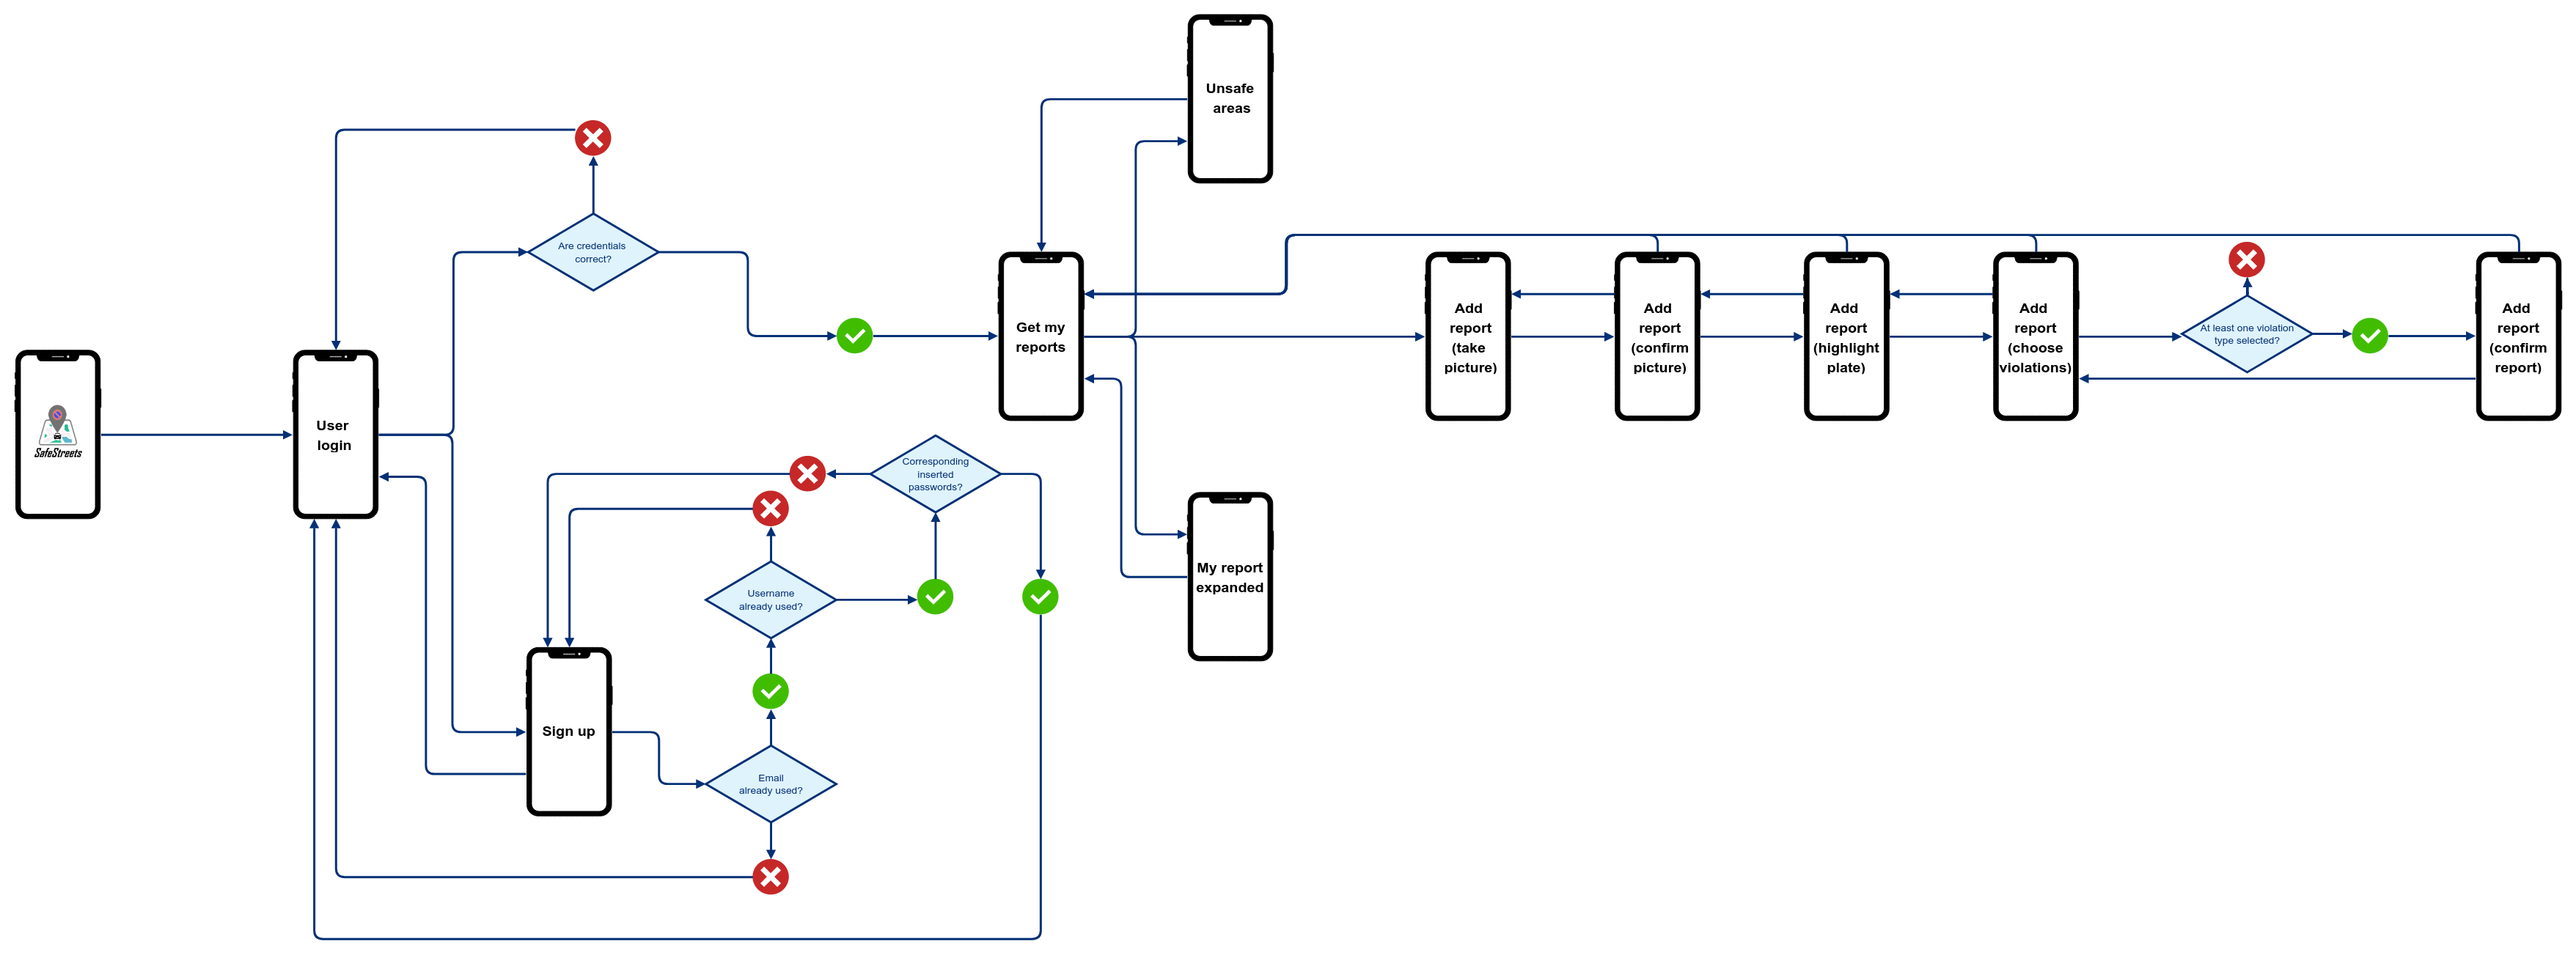
\includegraphics[width=\textwidth]{images/Flow/UserSimpleFlow}
			\end{figure}
			\clearpage
			\subsection{User flow with mockups}
			\begin{figure}[!h]
				\centering
				\includegraphics[width=\textwidth]{images/Flow/UserFlow}
			\end{figure}
		\clearpage
		\section{Authority flow}
			\paragraph{}
				This is the user experience seen in the perspective of an Authority
			\subsection{Authority logical flow}
			\begin{figure}[!h]
				\centering
				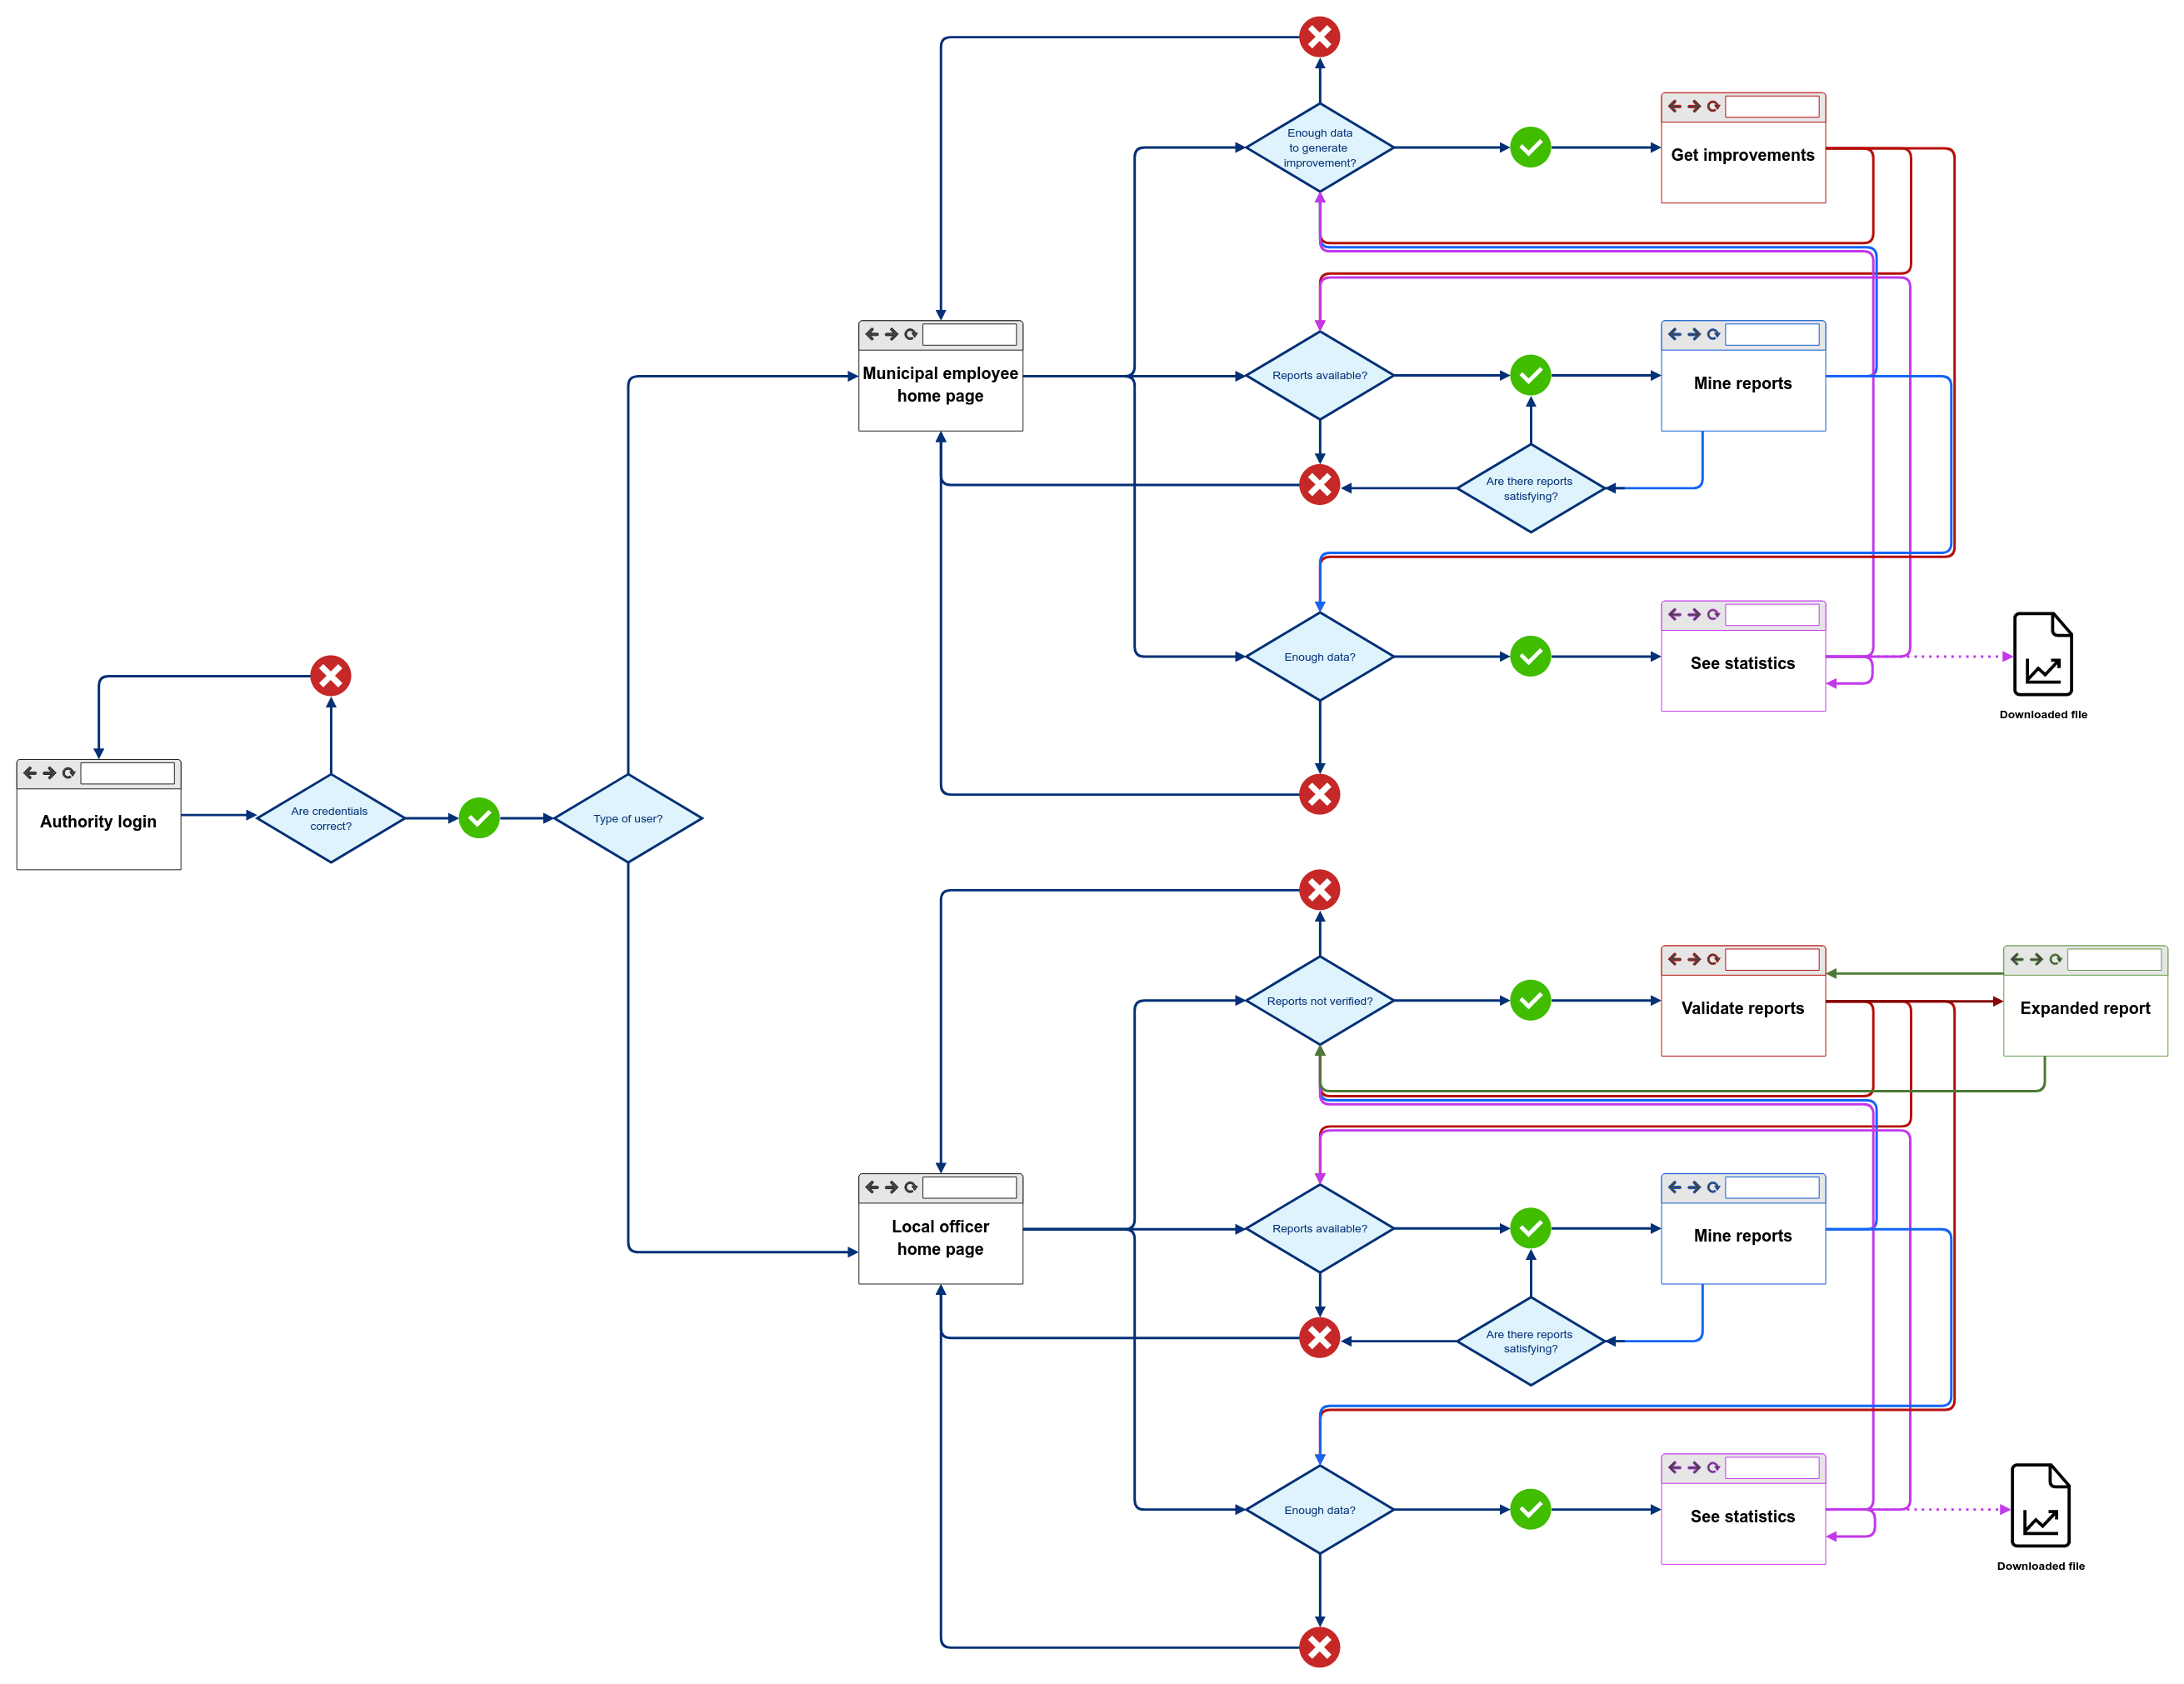
\includegraphics[width=\textwidth]{images/Flow/AuthoritySimpleFlow}
			\end{figure}
			\subsection{Authority flow with mockups}
			\begin{figure}[!h]
				\centering
				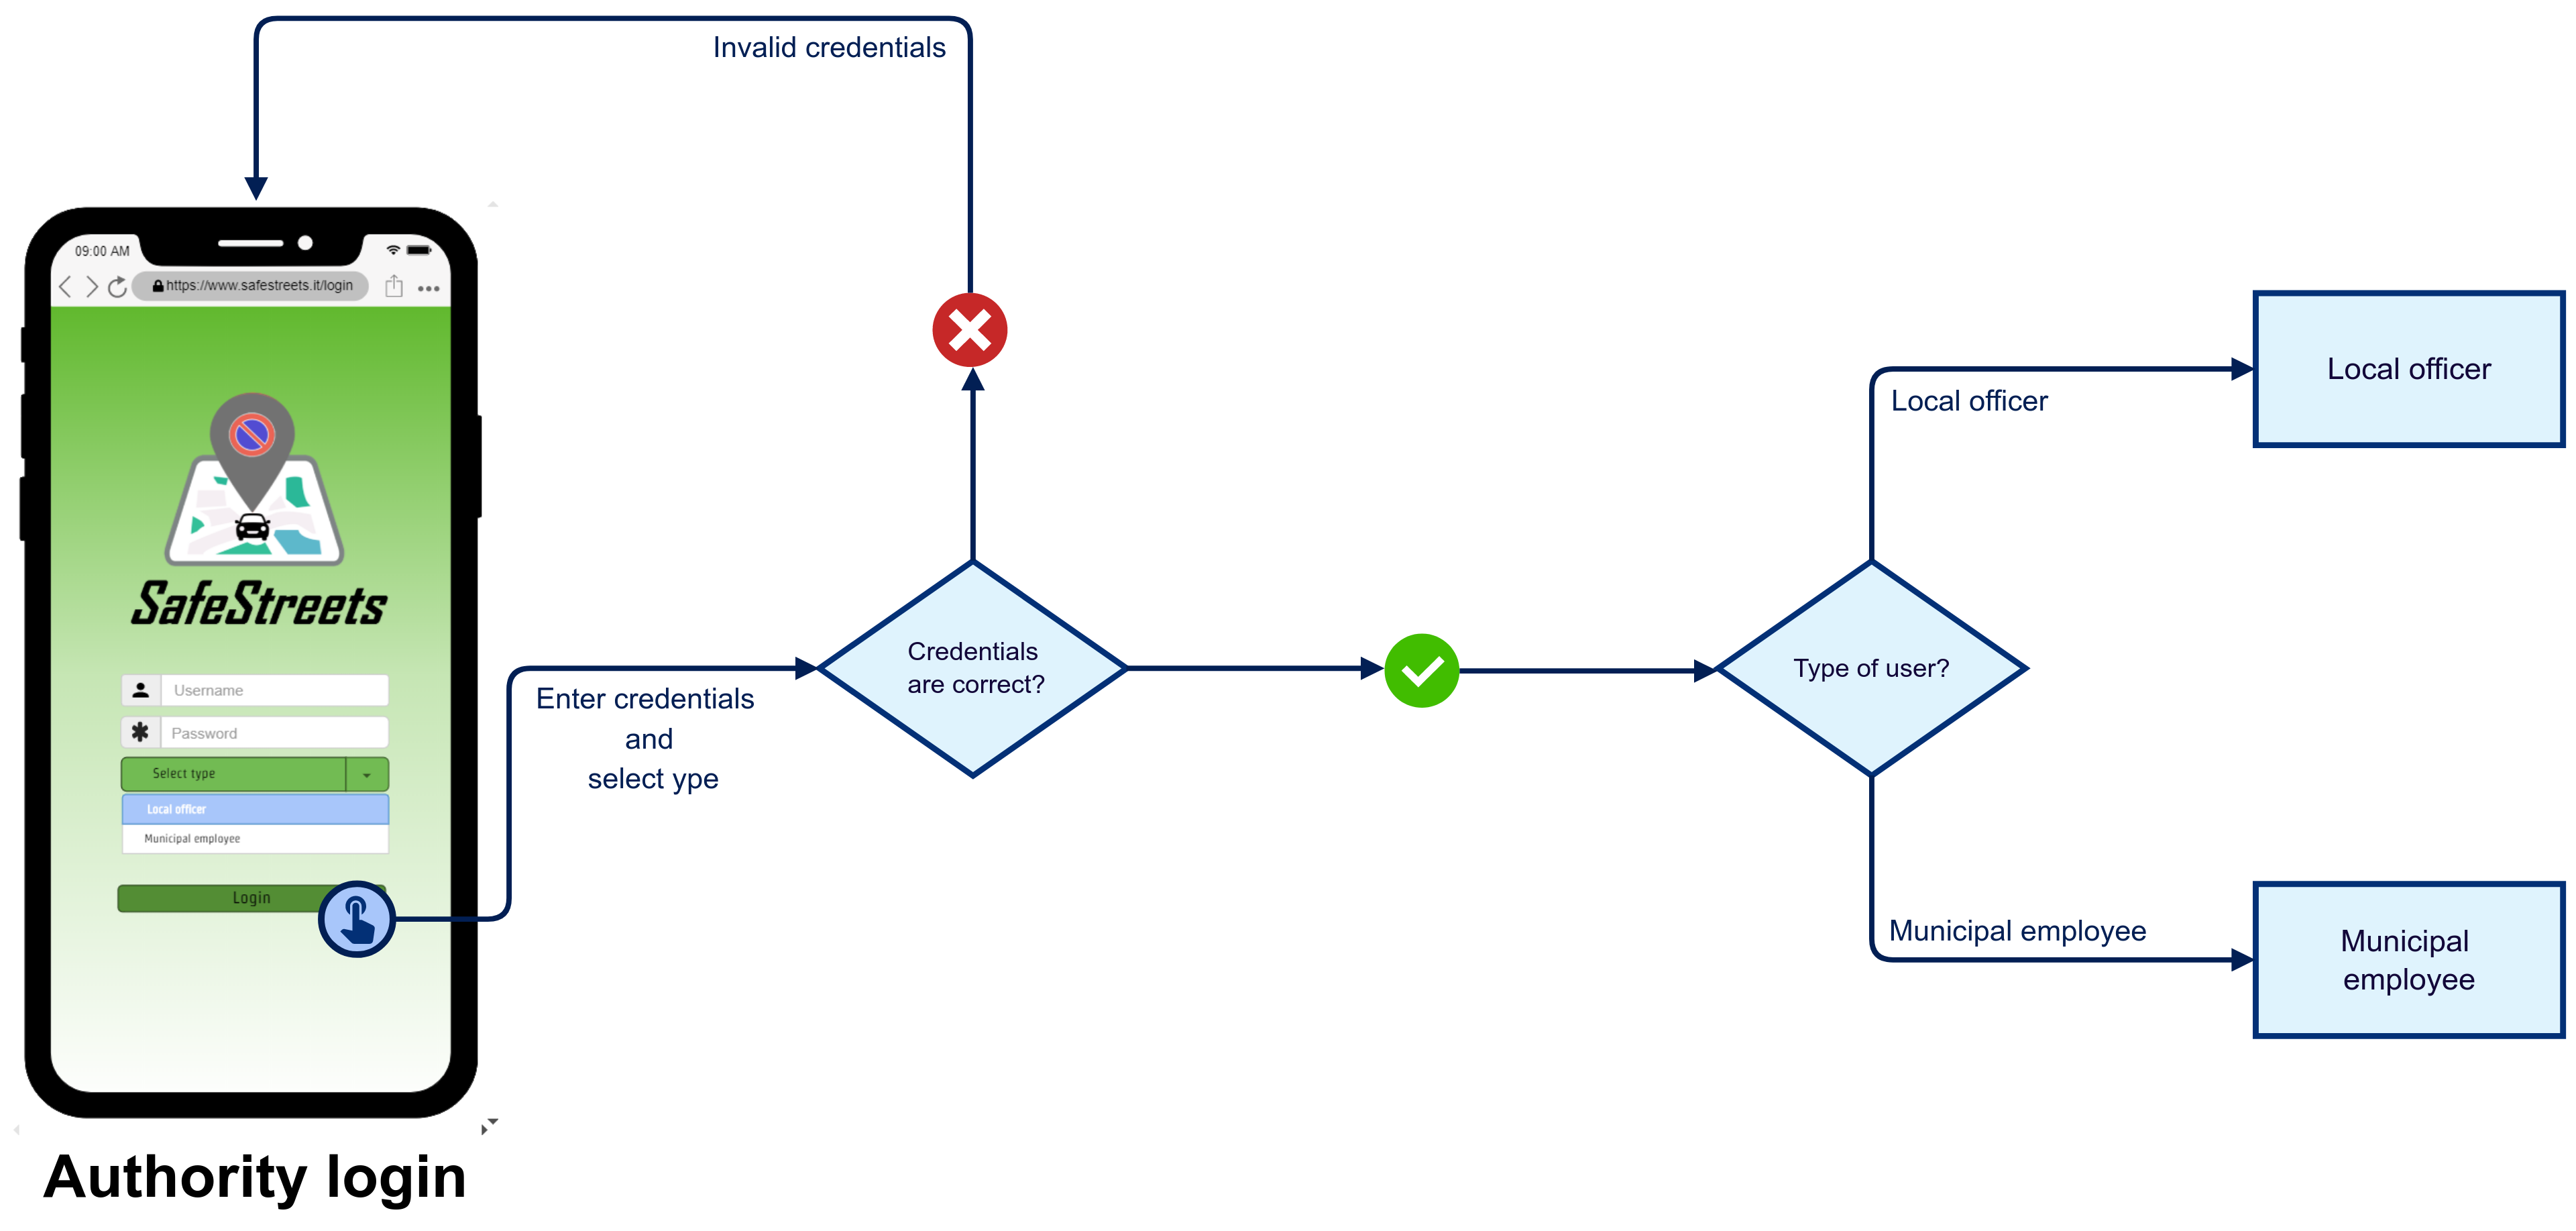
\includegraphics[width=\textwidth]{images/Flow/AuthorityFlow}
			\end{figure}
			\clearpage
			\subsection{Municipal Employee flow with mockups}
			\begin{figure}[!h]
				\centering
				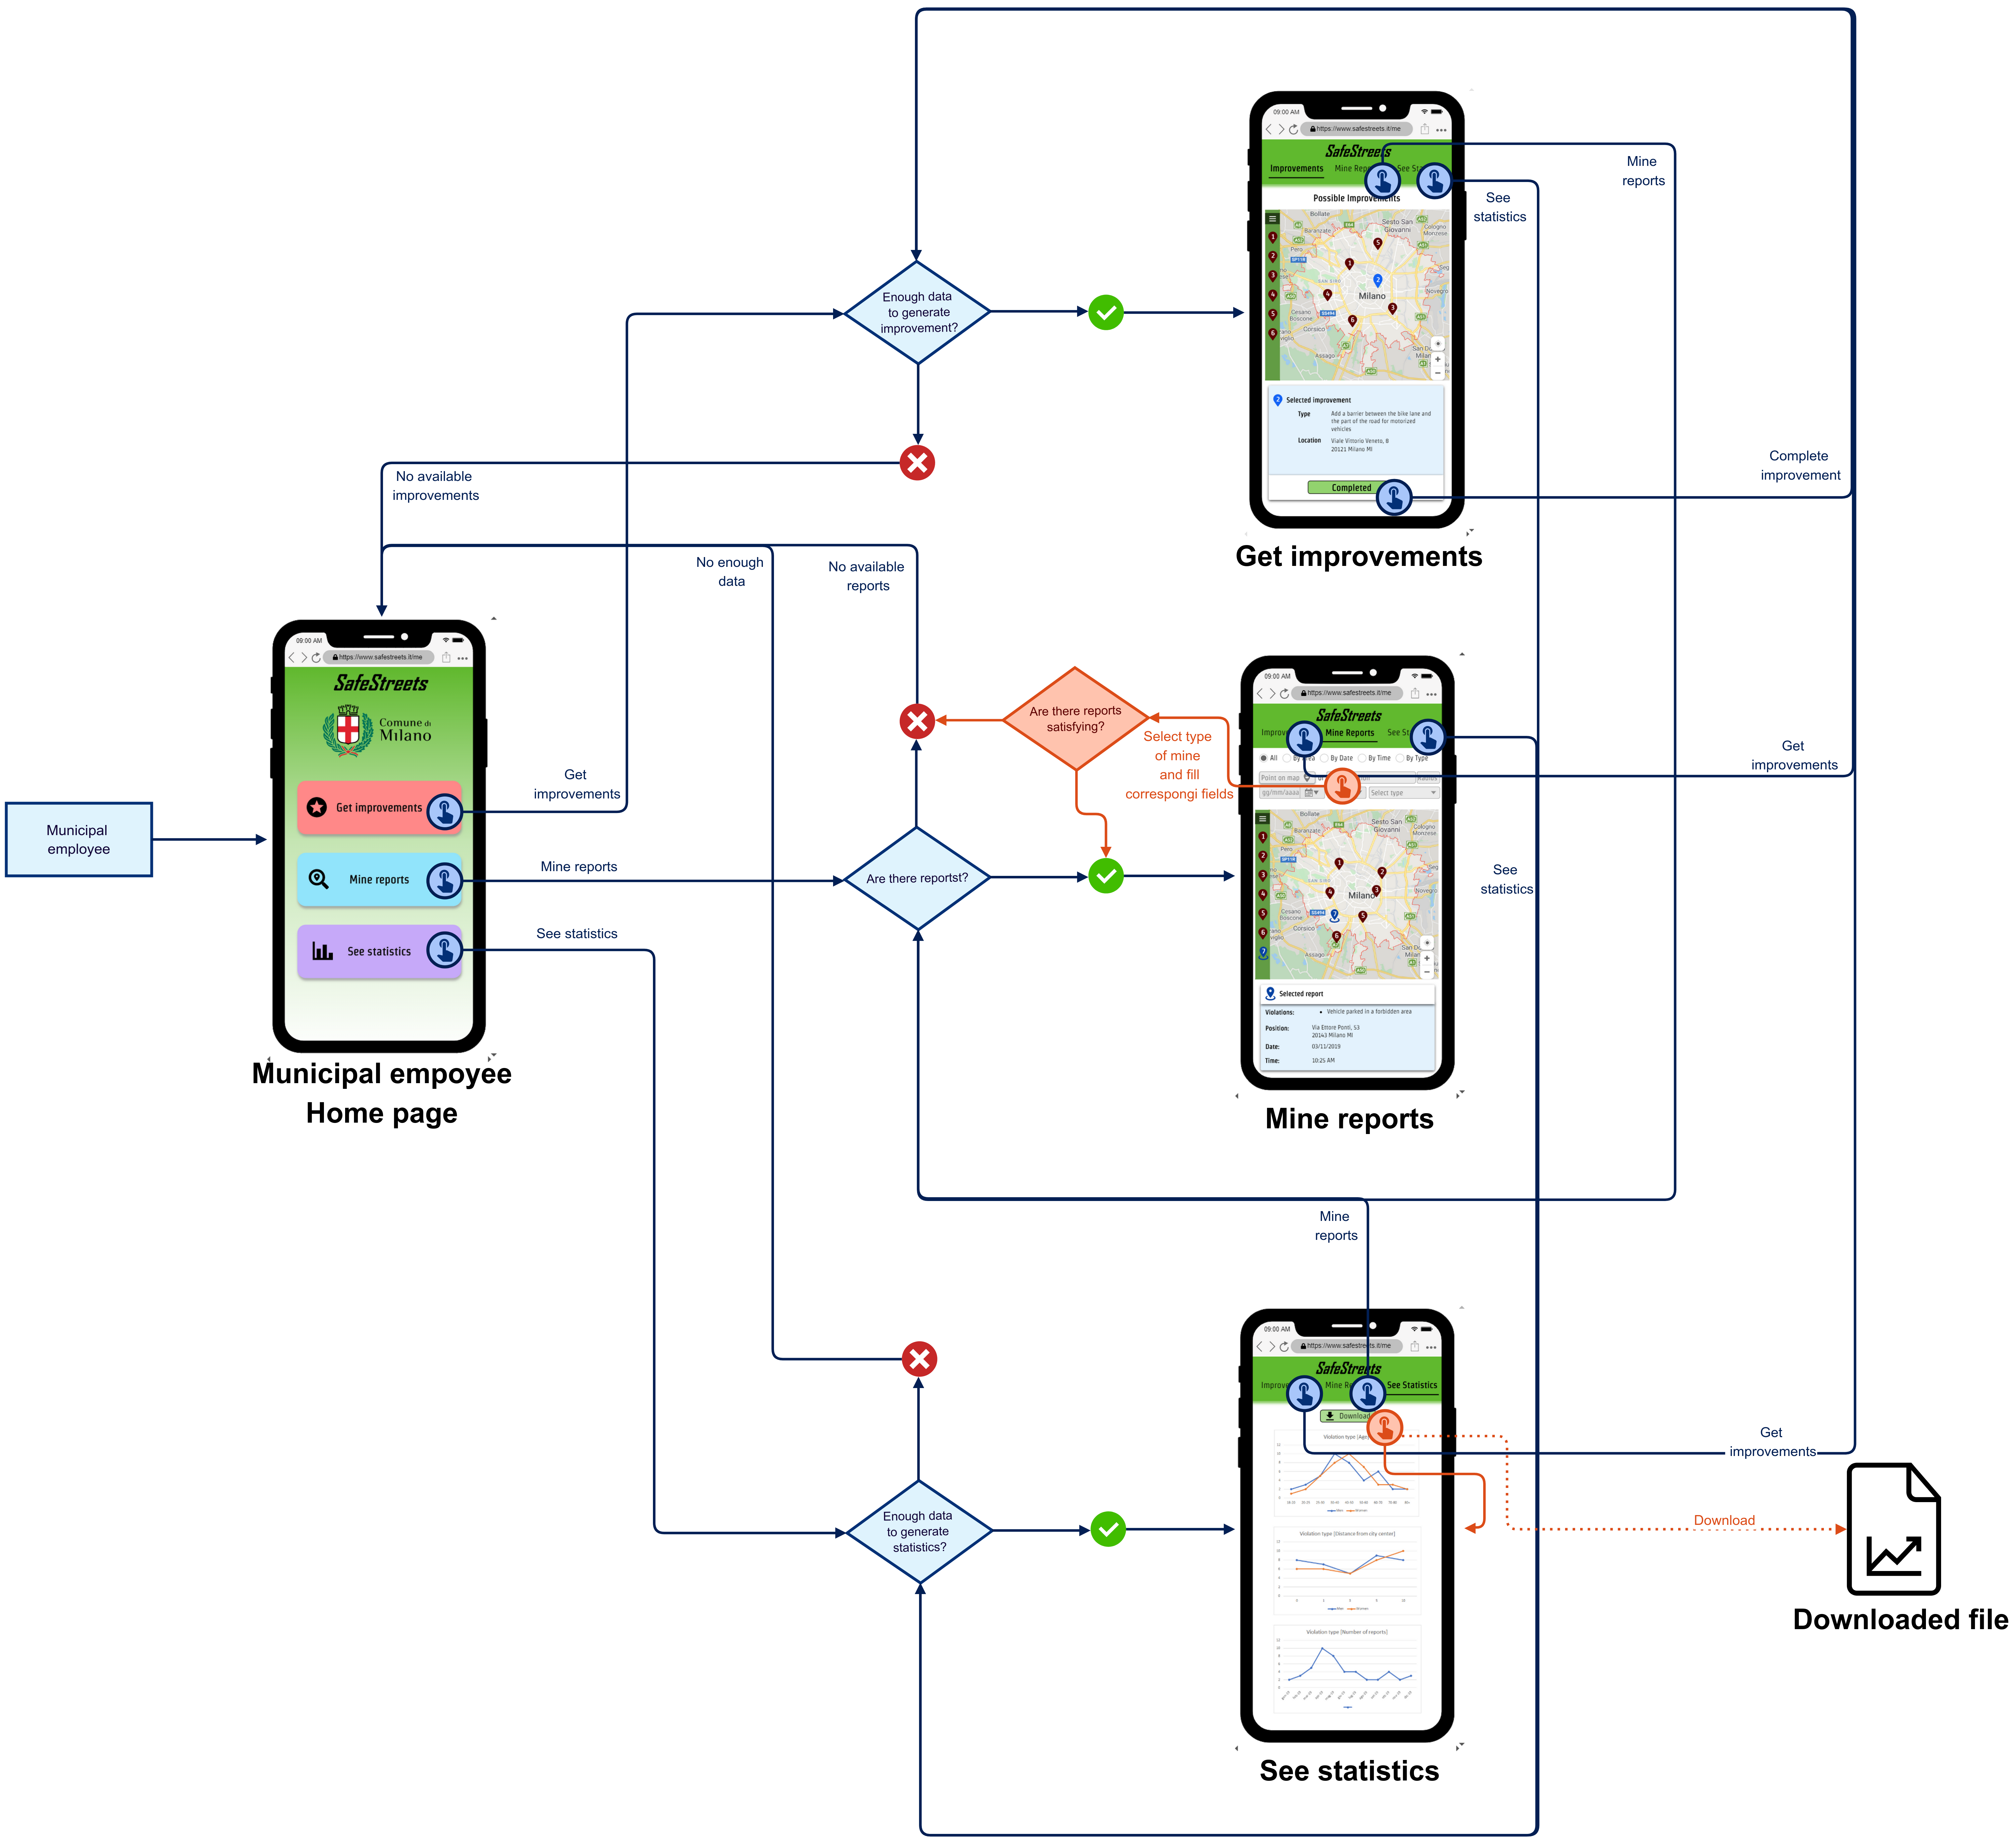
\includegraphics[width=\textwidth]{images/Flow/MEFlow}
			\end{figure}
			\clearpage
			\subsection{Local Officer flow with mockups}
			\begin{figure}[!h]
				\centering
				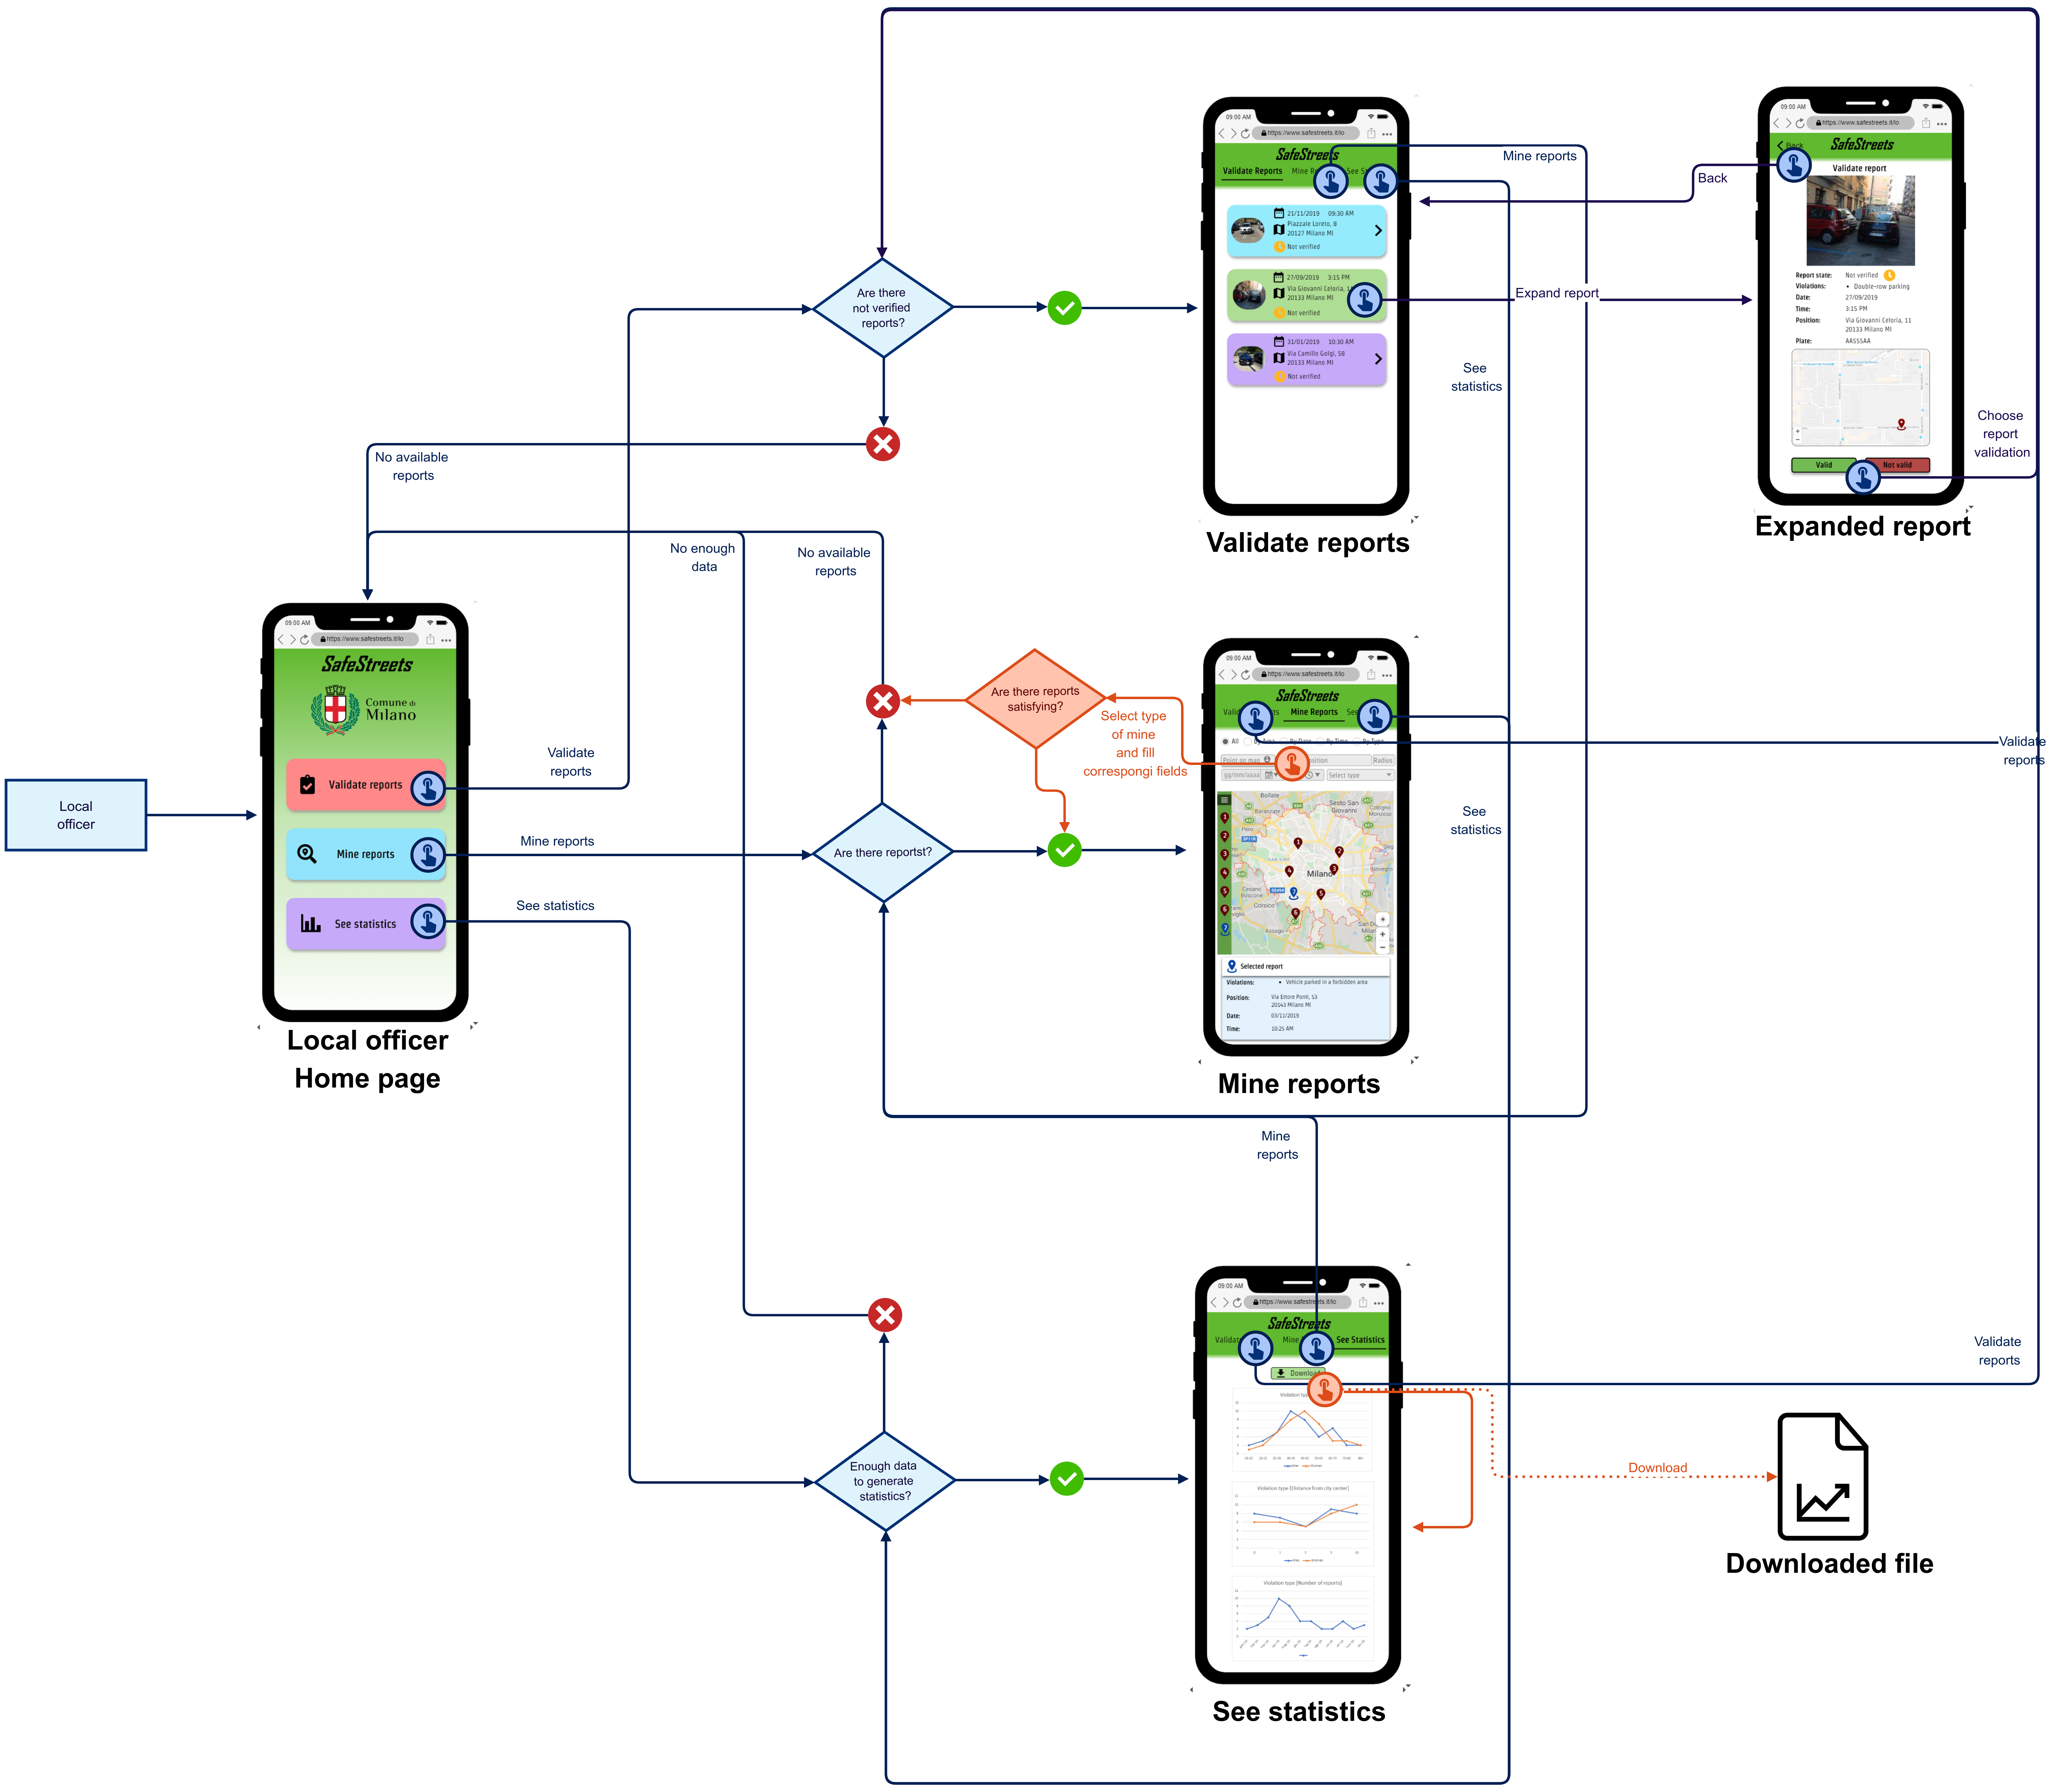
\includegraphics[width=\textwidth]{images/Flow/LOFlow}
			\end{figure}
		